\documentclass[12pt, man, natbib]{apa6}
\usepackage[USenglish]{babel}
\usepackage{setspace}
\usepackage{xcolor}
\usepackage{soul}
\usepackage{hyperref}

\title{Positioning the Phenomenon of Pipeline Spills in the Literature}
\shorttitle{Positioning}
\author{Julian Barg\\barg.julian@gmail.com}
\affiliation{Ivey Business School}
\setcitestyle{authoryear, open={()},close={)},citesep={,},aysep=}

\graphicspath {{figures/}}

% \abstract{}


\begin{document}
	
	\maketitle
	
	\singlespacing
	
	\section{}	
	
	The phenomenon of pipeline spills can be approached from different angles. Apart from learning, there is the angle of other organizations' responses to a focal firm's oil spill (especially from a network perspective). And there is a cross-sectional puzzle: what differentiates a pipeline operator that experiences many spills from one that experiences few? The learning perspective encompasses a longitudinal view: when or how does a pipeline operator improve its track record? 
	
	This last longitudinal story, which the learning angle encompasses, is attractive with regard to the motivation of such piece. We do already know that the environmental impacts exist, and we have a hunch that the response, save for a couple major incidents, is inadequate (since the responding actors have not been successful in ending the phenomenon of pipeline spills). If we were to take the current status quo as a starting point, we might end up with some implications that can be applied to the pipeline operator industry as it currently stands, implications that could yield some concrete medium term improvements over the current status quo\footnote{Although I am afraid we might just end up with an unimaginative statement along the lines of "Ey, we need enforcement, jo!"}.
	
	However, the learning literature is not a homogeneous entity. There are (at least) three different avenues from learning into pipeline safety, and eventually into environmental performance: (1) the effect of experience, (2) rare events (failures), and (3) population-level learning. Let's look at these three one at a time.
	
	\subsection{(1) The effect of experience}
	
	Learning is typically defined as "a change in [an] organization's knowledge [or behavior] that occurs as a function of experience" \citep[31]{Argote2013b}. With the interest of reducing oil spills in mind, it would be interesting to see whether as a function of experience (in operating pipelines), operations make headway in safety. Further, what attributes (of the focal organization or the environment) would aid or impede this learning process? However, the learning literature in this discourse (of learning as a function of cumulative experience) has taken an uncritical view so far. It is assumed an organization gets better at a task, the longer it performs the task. But what if this task is not "operating a pipeline safely", but rather "spilling oil and getting away with it"?
	
	\subsection{(2) Learning from rare events or learning from failure}
	
	Business as usual over an extended period of time might result in mindlessness and complacency, which squashes innovation and change. On the other hand individual, exceptional events can be path-breaking, if they are surprising in content and hold metaphorical power \citep{March1991}. For instance, individual smaller spills are quite frequent in the pipeline industry. They can easily be "rationalized away" by the operators, or may even be reinterpreted as successes ("we got the incident under control fast, and managed to keep the spill volume low").
	
	Very few oil spills have a disproportionate (relative to the median) spill volume; when those spills occur near a water way, the oil becomes difficult to recover, and the environmental impact can be enormous. While the average oil spill receives little to no coverage, larger oil spills might attain a lot of attention. Subsequently, stakeholders may pressure the operator and its peers to change their behavior. Or the oil spill may lead to high cost (e.g., through lawsuits) which other actors include in their risk analysis.  As a result of rare events, a cost-benefit analysis for action on pipeline safety might swing in favor of pipeline safety. Or the incident might result in a search process that leads to measures (for pipeline safety) being considered at all for the first time (the cost-benefit analysis might then just become a ceremony) \citep{Madsen2010}.
	
	\subsection{(3) Population-level learning}

	\begin{figure}
	\caption{Cumulative spill volume of largest pipeline spills}
	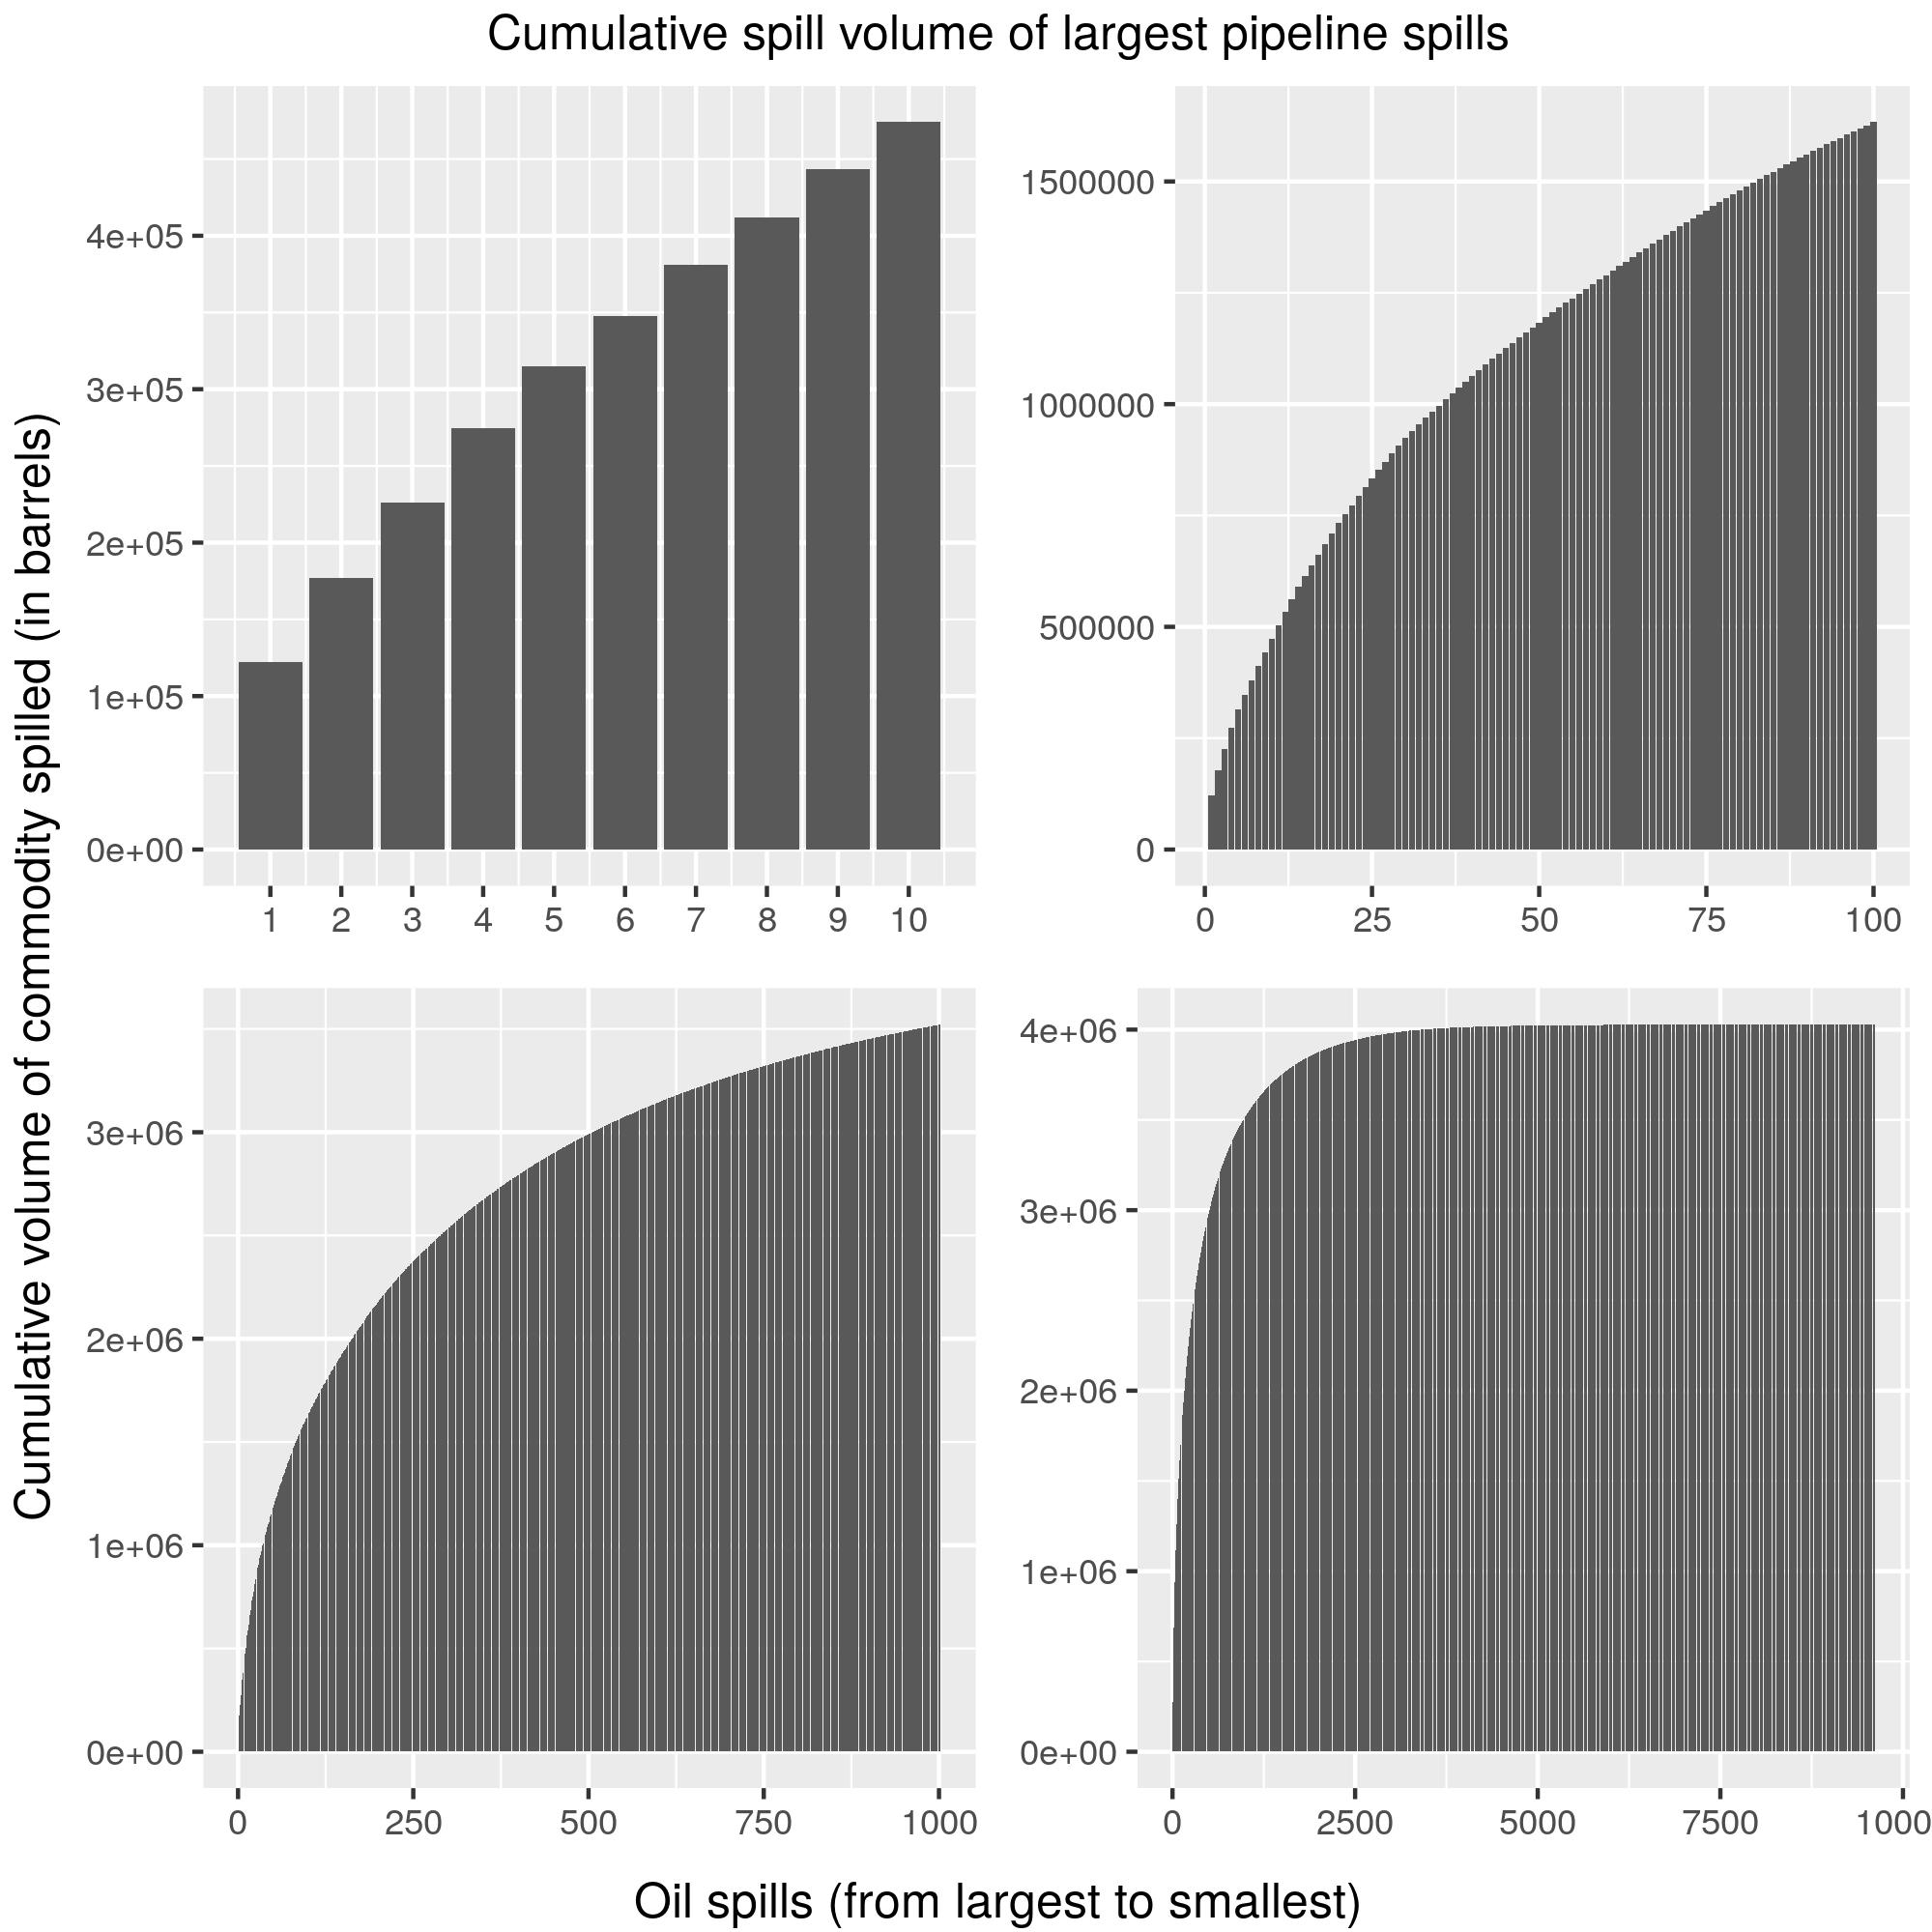
\includegraphics{figures/cumulative_spill_volume.jpg}
	\end{figure}
	 
	(3) Exhibit 1 shows that from an environmental perspective, we would not just care about the largest couple of incidents. Up until the 1000s or so incident, the cumulative spill volume from all spills is still increasing significantly. That does not contradict the previous point - individual events can be disproportionately important if they change the trajectory of a development.
	

	
\bibliography{bibliography}

\end{document}